\documentclass{standalone}

\usepackage{ tikz }
\usetikzlibrary{automata, positioning, arrows}

\begin{document}
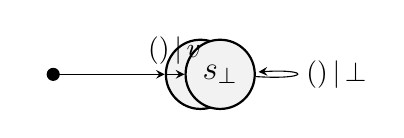
\begin{tikzpicture}[
        ->,
        >=stealth,
        node distance=0.25cm,
        every state/.style={font=\large, thick, fill=gray!10},
        initial text=$ $,
        initial distance=1.5cm,
        every initial by arrow/.style={*->},
        every edge/.append style={},
        yscale=-1,
        x=20pt,
        y=20pt
    ]
    \node[state, initial] (v) {\(s_v\)};
    \node[state, right of=v] (bot) {\(s_\bot\)};

    \draw (v) edge[above] node{\( () \,|\, v\)} (bot)
    (bot) edge[loop right] node{\( () \,|\, \bot\)} (bot)
    ;
\end{tikzpicture}
\end{document}